\documentclass{standalone}
\usepackage{tikz}
\usetikzlibrary{patterns, positioning}


\begin{document}
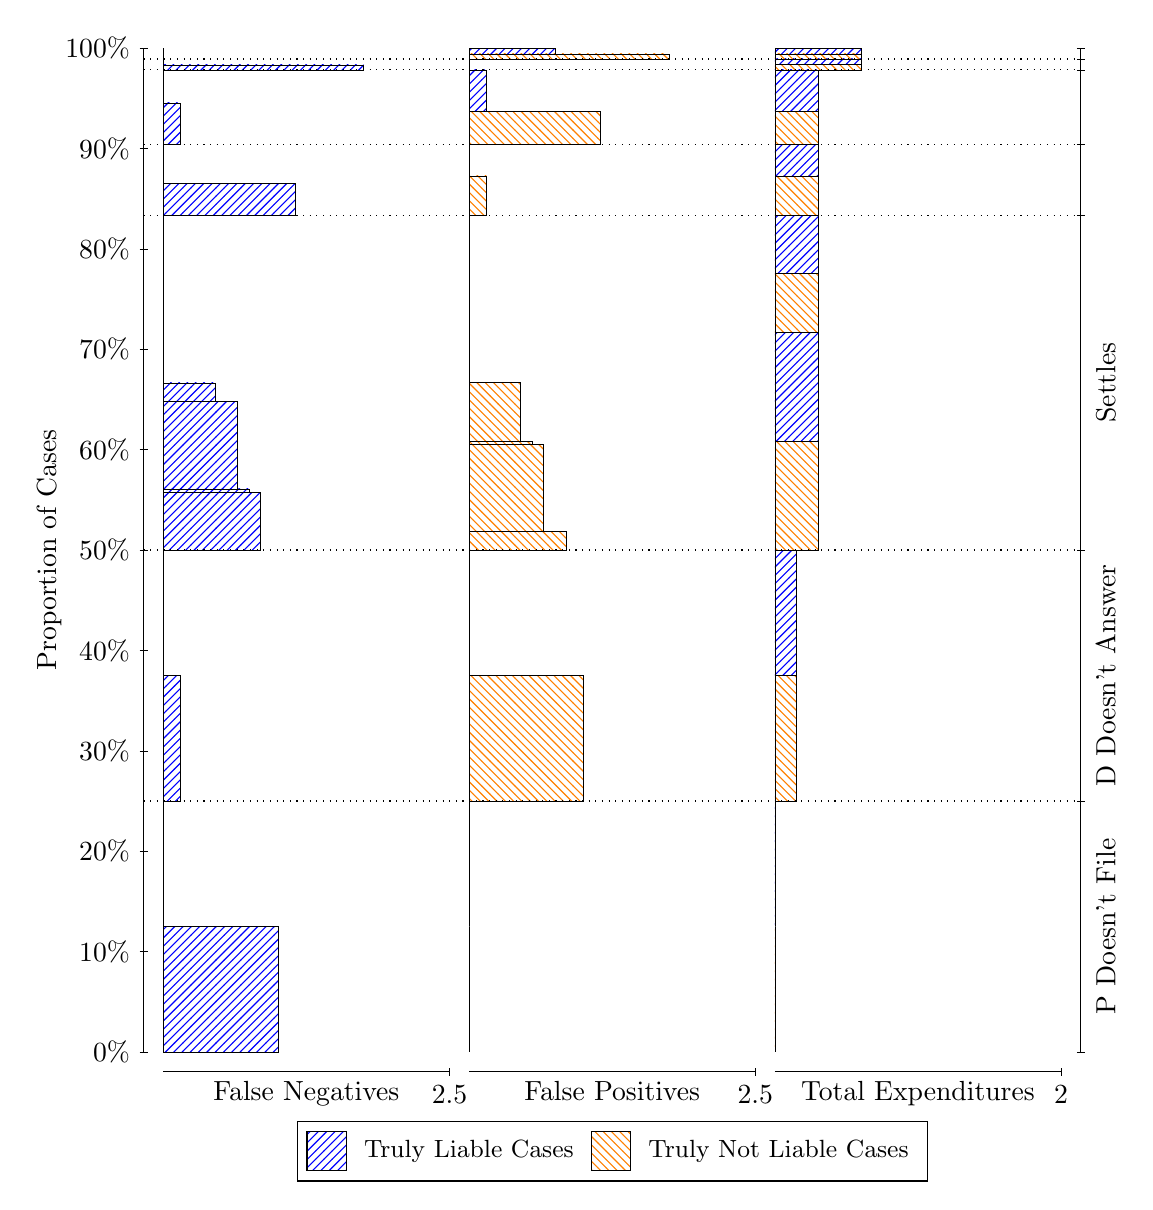
\begin{tikzpicture}
\draw[black, very thin] (1.5,1.75) -- (1.5,14.5);
\node[rotate=90, text=black, anchor=center] at (0.3, 8.125) {Proportion of Cases};
\draw[black, very thin] (1.45,1.75) -- (1.55,1.75);
\node[text=black, anchor=east] at (1.45, 1.75) {0\%};
\draw[black, very thin] (1.45,3.025) -- (1.55,3.025);
\node[text=black, anchor=east] at (1.45, 3.025) {10\%};
\draw[black, very thin] (1.45,4.3) -- (1.55,4.3);
\node[text=black, anchor=east] at (1.45, 4.3) {20\%};
\draw[black, very thin] (1.45,5.575) -- (1.55,5.575);
\node[text=black, anchor=east] at (1.45, 5.575) {30\%};
\draw[black, very thin] (1.45,6.85) -- (1.55,6.85);
\node[text=black, anchor=east] at (1.45, 6.85) {40\%};
\draw[black, very thin] (1.45,8.125) -- (1.55,8.125);
\node[text=black, anchor=east] at (1.45, 8.125) {50\%};
\draw[black, very thin] (1.45,9.4) -- (1.55,9.4);
\node[text=black, anchor=east] at (1.45, 9.4) {60\%};
\draw[black, very thin] (1.45,10.675) -- (1.55,10.675);
\node[text=black, anchor=east] at (1.45, 10.675) {70\%};
\draw[black, very thin] (1.45,11.95) -- (1.55,11.95);
\node[text=black, anchor=east] at (1.45, 11.95) {80\%};
\draw[black, very thin] (1.45,13.225) -- (1.55,13.225);
\node[text=black, anchor=east] at (1.45, 13.225) {90\%};
\draw[black, very thin] (1.45,14.5) -- (1.55,14.5);
\node[text=black, anchor=east] at (1.45, 14.5) {100\%};

\draw[black, very thin] (13.4,1.75) -- (13.4,14.5);
\draw[black, very thin] (13.35,1.75) -- (13.45,1.75);
\node[anchor=west] at (13.35, 1.75) {};
\draw[black, very thin] (13.35,4.9375) -- (13.45,4.9375);
\node[anchor=west] at (13.35, 4.9375) {};
\draw[black, very thin] (13.35,8.125) -- (13.45,8.125);
\node[anchor=west] at (13.35, 8.125) {};
\draw[black, very thin] (13.35,12.377) -- (13.45,12.377);
\node[anchor=west] at (13.35, 12.377) {};
\draw[black, very thin] (13.35,13.28) -- (13.45,13.28);
\node[anchor=west] at (13.35, 13.28) {};
\draw[black, very thin] (13.35,14.222) -- (13.45,14.222);
\node[anchor=west] at (13.35, 14.222) {};
\draw[black, very thin] (13.35,14.361) -- (13.45,14.361);
\node[anchor=west] at (13.35, 14.361) {};
\draw[black, very thin] (13.35,14.5) -- (13.45,14.5);
\node[anchor=west] at (13.35, 14.5) {};

\draw[black, very thin, pattern color=blue, pattern=north east lines] (1.75,1.75) rectangle (3.2033,3.3437);
\draw[black, very thin, pattern color=orange, pattern=north west lines] (1.75,3.3437) rectangle (1.75,4.9375);
\draw[black, very thin, pattern color=blue, pattern=north east lines] (1.75,4.9375) rectangle (1.968,6.5312);
\draw[black, very thin, pattern color=orange, pattern=north west lines] (1.75,6.5312) rectangle (1.75,8.125);
\draw[black, very thin, pattern color=blue, pattern=north east lines] (1.75,8.125) rectangle (2.9853,8.8592);
\draw[black, very thin, pattern color=blue, pattern=north east lines] (1.75,8.8592) rectangle (2.84,8.9012);
\draw[black, very thin, pattern color=blue, pattern=north east lines] (1.75,8.9012) rectangle (2.6947,10.01);
\draw[black, very thin, pattern color=blue, pattern=north east lines] (1.75,10.01) rectangle (2.404,10.246);
\draw[black, very thin, pattern color=orange, pattern=north west lines] (1.75,10.246) rectangle (1.75,12.377);
\draw[black, very thin, pattern color=blue, pattern=north east lines] (1.75,12.377) rectangle (3.4213,12.779);
\draw[black, very thin, pattern color=orange, pattern=north west lines] (1.75,12.779) rectangle (1.75,13.28);
\draw[black, very thin, pattern color=blue, pattern=north east lines] (1.75,13.28) rectangle (1.968,13.804);
\draw[black, very thin, pattern color=orange, pattern=north west lines] (1.75,13.804) rectangle (1.75,14.222);
\draw[black, very thin, pattern color=blue, pattern=north east lines] (1.75,14.222) rectangle (4.2933,14.286);
\draw[black, very thin, pattern color=orange, pattern=north west lines] (1.75,14.286) rectangle (1.75,14.361);
\draw[black, very thin, pattern color=orange, pattern=north west lines] (1.75,14.361) rectangle (1.75,14.425);
\draw[black, very thin, pattern color=blue, pattern=north east lines] (1.75,14.425) rectangle (1.75,14.5);
\draw[black, very thin, pattern color=orange, pattern=north west lines] (5.6333,1.75) rectangle (5.6333,3.3438);
\draw[black, very thin, pattern color=blue, pattern=north east lines] (5.6333,3.3438) rectangle (5.6333,4.9375);
\draw[black, very thin, pattern color=orange, pattern=north west lines] (5.6333,4.9375) rectangle (7.0867,6.5313);
\draw[black, very thin, pattern color=blue, pattern=north east lines] (5.6333,6.5313) rectangle (5.6333,8.125);
\draw[black, very thin, pattern color=orange, pattern=north west lines] (5.6333,8.125) rectangle (6.8687,8.3578);
\draw[black, very thin, pattern color=orange, pattern=north west lines] (5.6333,8.3578) rectangle (6.578,9.4677);
\draw[black, very thin, pattern color=orange, pattern=north west lines] (5.6333,9.4677) rectangle (6.4327,9.5039);
\draw[black, very thin, pattern color=orange, pattern=north west lines] (5.6333,9.5039) rectangle (6.2873,10.255);
\draw[black, very thin, pattern color=blue, pattern=north east lines] (5.6333,10.255) rectangle (5.6333,12.377);
\draw[black, very thin, pattern color=orange, pattern=north west lines] (5.6333,12.377) rectangle (5.8513,12.877);
\draw[black, very thin, pattern color=blue, pattern=north east lines] (5.6333,12.877) rectangle (5.6333,13.28);
\draw[black, very thin, pattern color=orange, pattern=north west lines] (5.6333,13.28) rectangle (7.3047,13.698);
\draw[black, very thin, pattern color=blue, pattern=north east lines] (5.6333,13.698) rectangle (5.8513,14.222);
\draw[black, very thin, pattern color=orange, pattern=north west lines] (5.6333,14.222) rectangle (5.6333,14.297);
\draw[black, very thin, pattern color=blue, pattern=north east lines] (5.6333,14.297) rectangle (5.6333,14.361);
\draw[black, very thin, pattern color=orange, pattern=north west lines] (5.6333,14.361) rectangle (8.1767,14.425);
\draw[black, very thin, pattern color=blue, pattern=north east lines] (5.6333,14.425) rectangle (6.7233,14.5);
\draw[black, very thin, pattern color=orange, pattern=north west lines] (9.5167,1.75) rectangle (9.5167,3.3438);
\draw[black, very thin, pattern color=blue, pattern=north east lines] (9.5167,3.3438) rectangle (9.5167,4.9375);
\draw[black, very thin, pattern color=orange, pattern=north west lines] (9.5167,4.9375) rectangle (9.7892,6.5313);
\draw[black, very thin, pattern color=blue, pattern=north east lines] (9.5167,6.5313) rectangle (9.7892,8.125);
\draw[black, very thin, pattern color=orange, pattern=north west lines] (9.5167,8.125) rectangle (10.062,9.5039);
\draw[black, very thin, pattern color=blue, pattern=north east lines] (9.5167,9.5039) rectangle (10.062,10.891);
\draw[black, very thin, pattern color=orange, pattern=north west lines] (9.5167,10.891) rectangle (10.062,11.642);
\draw[black, very thin, pattern color=blue, pattern=north east lines] (9.5167,11.642) rectangle (10.062,12.377);
\draw[black, very thin, pattern color=orange, pattern=north west lines] (9.5167,12.377) rectangle (10.062,12.877);
\draw[black, very thin, pattern color=blue, pattern=north east lines] (9.5167,12.877) rectangle (10.062,13.28);
\draw[black, very thin, pattern color=orange, pattern=north west lines] (9.5167,13.28) rectangle (10.062,13.698);
\draw[black, very thin, pattern color=blue, pattern=north east lines] (9.5167,13.698) rectangle (10.062,14.222);
\draw[black, very thin, pattern color=orange, pattern=north west lines] (9.5167,14.222) rectangle (10.607,14.297);
\draw[black, very thin, pattern color=blue, pattern=north east lines] (9.5167,14.297) rectangle (10.607,14.361);
\draw[black, very thin, pattern color=orange, pattern=north west lines] (9.5167,14.361) rectangle (10.607,14.425);
\draw[black, very thin, pattern color=blue, pattern=north east lines] (9.5167,14.425) rectangle (10.607,14.5);
\draw[black, dotted] (1.5,4.9375) -- (13.4,4.9375);
\draw[black, dotted] (1.5,8.125) -- (13.4,8.125);
\draw[black, dotted] (1.5,12.377) -- (13.4,12.377);
\draw[black, dotted] (1.5,13.28) -- (13.4,13.28);
\draw[black, dotted] (1.5,14.222) -- (13.4,14.222);
\draw[black, dotted] (1.5,14.361) -- (13.4,14.361);
\draw[black, very thin] (1.75,1.5) -- (5.3833,1.5);
\node[text=black, anchor=north] at (3.5667, 1.5) {False Negatives};
\draw[black, very thin] (5.3833,1.45) -- (5.3833,1.55);
\node[text=black, anchor=north] at (5.3833, 1.45) {2.5};

\draw[black, very thin] (5.6333,1.5) -- (9.2667,1.5);
\node[text=black, anchor=north] at (7.45, 1.5) {False Positives};
\draw[black, very thin] (9.2667,1.45) -- (9.2667,1.55);
\node[text=black, anchor=north] at (9.2667, 1.45) {2.5};

\draw[black, very thin] (9.5167,1.5) -- (13.15,1.5);
\node[text=black, anchor=north] at (11.333, 1.5) {Total Expenditures};
\draw[black, very thin] (13.15,1.45) -- (13.15,1.55);
\node[text=black, anchor=north] at (13.15, 1.45) {2};

\node[text=black, centered, rotate=90] at (13.72, 3.3437) {P Doesn't File};
\node[text=black, centered, rotate=90] at (13.72, 6.5312) {D Doesn't Answer};
\node[text=black, centered, rotate=90] at (13.72, 10.251) {Settles};





\draw (7.449999999999999,1.5) node[draw=none] (baseCoordinate) {};
\begin{scope}[align=center]
        \matrix[scale=0.5, draw=black, below=0.5cm of baseCoordinate, nodes={draw}, column sep=0.1cm]{
            \node[rectangle, draw, minimum width=0.5cm, minimum height=0.5cm, pattern color=blue, pattern=north east lines] {}; &
            \node[draw=none, font=\small, text=black] (B) {Truly Liable Cases}; &
            \node[rectangle, draw, minimum width=0.5cm, minimum height=0.5cm, pattern color=orange, pattern=north west lines] {}; &
            \node[draw=none, font=\small, text=black] (B) {Truly Not Liable Cases}; \\
            };
\end{scope}

\end{tikzpicture}
\end{document}